%Started on Monday 28 August 2006
%Aug: 29, 30
%Sep:  7,  8, 13
% 2007
%Feb:  4
%Mar:  8, 18, 19, 20, 28, 30
%Apr:  2,  3,  4,  5, 18, 21

%
% Chapter: Warm-start
%
\label{ch:Warmstart}

In this chapter we develop an efficient way of constructing a 
starting point for structured large-scale stochastic linear programs.
We first present the relevant
concepts of stochastic programming and review some studies on 
warm-start techniques for interior point methods. Then we introduce 
the proposed method of generating an advanced starting point for 
stochastic programming that exploits the inherent structure of the
problem. Finally, we present an analysis of the warm-start strategy.
The results presented in this chapter have been the subject
of a joint work with Jacek Gondzio and Andreas Grothey
\cite{ColomboGondzioGrothey06}. 


%
% Section
%
\section{Stochastic programming}

Stochastic programming \cite{BirgeLouveaux,KallWallace}
is a technique to help decision-making 
in many areas of applied mathematics, logistics, engineering, economics and 
finance where some parameters are unknown.

\ignore{
In a large scenario tree there may be very little difference among 
scenarios, and so the large-scale problem can provide a fine-grained 
solution to a problem that could have been solved more coarsely by 
using a much smaller tree. This observation suggests a
warm-start technique that can be applied in the context of interior 
point methods. A warm-start solution is obtained by solving the 
stochastic optimization problem for a reduced event tree, the dimension
of which is much smaller than that of the complete one. The solution 
to the reduced problem is used to construct an advanced iterate for 
the complete formulation. We provide evidence that this novel way 
of exploiting the problem structure to generate an initial iterate
provides a better starting point (in terms of centrality, feasibility, 
and closeness to optimality) than the one produced by a generic 
strategy.
}

By stochastic programming, we mean decision and control models in which 
data evolves over time, and are subject to significant uncertainty.
%
Uncertainty in the data is a commonly observed phenomenon in
optimization problems coming from applications. Uncertainty
affects problems that aim to plan future actions based on forecasted
prices or costs. In can be argued that nearly all practical
optimization problems display uncertainty in the data, even if this is
not made explicit in the chosen solution method. 

\ignore{
A crude approach to the problem of optimization under uncertainty
has been to replace the uncertain data by their expected value and
solve an {\em average case} problem. However, this approach is not
suitable when some sort of provision of hedging against risk has to be
taken into account. Another popular approach is {\em Robust
optimization}, or the optimization of the {\em worst case}
scenario \cite{KallWallace}. 
}

When the uncertainty cannot be conveniently forecasted, the use of 
deterministic models is considered inadequate for decision making. In 
these situations, being able to describe and model the uncertain parameters
becomes a requirement for robust decision making. Stochastic 
programming is the discipline that 
studies the methods and provides the tools for modelling uncertainty.

Stochastic programming models uncertainty through the analysis 
of possible future outcomes (scenarios). 
As the robustness of the decisions taken increases with the detail of the 
description, this encourages the generation of very large scenario trees.
Stochastic programming aims to take all possible future scenarios 
into account, weighting them
with their respective probabilities. Its strength lies in the
adaptability which allows to express preferences such as restricting
the exposure to risk. Unlike alternative approaches, it allows to model
situations in which possible future events are correlated or follow a
time-structure, in that realisations become known in stages and it is
possible to react to the observed events.

Taking into account a large number of possible scenarios leads
to the generation of large-scale structured optimization problems.
With the growing industrial acknowledgement of the benefits of 
considering uncertainty for planning purposes, it is expected that the 
need for solving very large instances will grow as well.

Its perceived weaknesses are the need for reliable forecasts
of the probabilities of the future events under consideration
(which may not be available), and the fact that stochastic programming
(especially when applied to multi-stage models) tends to lead to
problems with very large dimensions, thus making their solution
challenging. 

As the dimensions of the problems increase, the computational advantages 
of relying on interior point solvers become more and more evident. 
Very-large-scale problems, however, create more than one difficulty to general 
purpose solvers.
Problems of such sizes can be solved provided they are not only sparse,
but also structured. If that is the case, then the structure present 
in the matrix should be conveniently exploited.
The easier access to powerful parallel machines leads to a 
further advantage coming from assigning the computational work 
to more than one processing unit through the parallelisation of 
the linear algebra.
This is where structure-exploiting parallel solvers such as \OOPS 
\cite{GondzioSarkissian} excel. Moreover, structure-exploiting interior 
point methods can be used not only for linear programming problems, 
but also for quadratic and nonlinear problems \cite{GondzioGrothey07}.

%
%
\subsection{Stochastic programming concepts}

A stochastic programming problem incorporates the uncertain parameters
in the model. 
Following \cite{BirgeLouveaux}, this can be illustrated by the 
{\em two-stage stochastic problem}
%
\be  \label{eq:SP1}
  \begin{array}{rl}
    \min        & c^T x + \E_\xi Q(x, \xi) \\
    \mbox{s.t.} & Ax = b,  \\
                & x\geq 0, \\
  \end{array}
\ee
%
where $\xi$ is a random variable and $\E_\xi$ is the expectation function
and
\be  \label{eq:SP2}
  \begin{array}{rcrl}
  Q(x, \xi) &\!\!\! = \!\!\! & \min & q(\xi)^T y(\xi) \\
            &   & \mbox{s.t.} & Wy(\xi) = h(\xi) - T(\xi)x, \\
	    &   &             & y(\xi) \ge 0.
  \end{array}
\ee
This can be interpreted as an optimization
problem in which some parameters or coefficients are unknown.
While (\ref{eq:SP1}) models the first stage decisions, 
(\ref{eq:SP2}) refers to the second stage decisions, which can
be made only after a realisation of the random variable $\xi$
has become known. Note how the first-stage decision variables $x$ 
appear in (\ref{eq:SP2}): at the time when the realisation
become available, the first-stage decisions have already been made.

\ignore{
Formulation (\ref{eq:SP}) is however an unsatisfactory model, since
it is unclear how to interpret the probabilistic constraint
$g(x,\xi) \le 0$. A better formulation is the stochastic program
with recourse:
\begin{eqnarray} \label{eq:SPRecourse}
\min_x \hspace{-1.5em} && \E_\xi[f(x, \xi) + Q(x, \xi)] \nonumber \\ 
  && Q(x,\xi) = \min_y \{\, q(y) : u_i(y) \ge g_i^+(x, \xi),\:\forall i \,\},\\
  && g_i^+(x, \xi) = \max \{\, g_i(x, \xi), \, 0 \,\}. \nonumber
\end{eqnarray}
}

In stochastic programming, the uncertain environment is 
described through a stochastic process which is assumed to be 
known or can be either estimated from historical data or 
conjectured according to some prescribed properties. The 
continuous process $\xi$ is usually further approximated by a discrete 
distribution, $\xi \in \{\xi_1, \ldots,\xi_n\}$, $p(\xi=\xi_i) = p_i$,
in order to obtain a computationally amenable description. 
%
In such a case, the most common techniques generate a 
finite, but usually very large, number of scenarios that represent an 
approximate description of the possible outcomes.

%The decision variables $x$ are
%split depending on the timing of the decision: $x_0$ are those
%variables whose value is to be decided {\em before} the random event
%becomes known, $x_i$ are decisions taken as a reaction to the outcome
%of $\xi$ being $\xi_i$ (recourse action). Problem
%(\ref{continuousSP}) then becomes
%\begin{equation}
%\min_{x} \sum_{i=1}^n p_i f(x_0, x_i, \xi_i)) \text{~subject
%to~}c(x_0, x_i, \xi_i) \le 0,
%\label{SP}
%\end{equation}

The model can be generalised to a {\em multi-stage model} in which 
the evolution of uncertainties can be 
described as an alternating sequence of decisions and random 
realisations that occur at different stages.
A multi-stage stochastic program with recourse is a multi-period 
mathematical program where parameters are assumed to be uncertain 
along the time path.

The stages do not necessarily refer to time periods, but they correspond
to steps in the decision process. In particular, at each stage the
realisations of some random parameters become known, and a decision
must be taken.
The main interest lies in the 
first-stage decisions which consist of all decisions that have to
be made before the information is revealed. Later-stage decisions 
are allowed to adapt to the information that has become available 
up to that point.

The discrete stochastic process can be represented as an 
{\em event tree} $\Ctree$,
where each node denotes a stage when a realisation 
of the random process becomes known and a subsequent decision is taken.
A path from the root to a leaf node of the event tree represents a 
scenario.
A very simple event tree is shown in Figure~\ref{fig:EventTree}.
%
\begin{figure}[ht]
  \begin{center}
    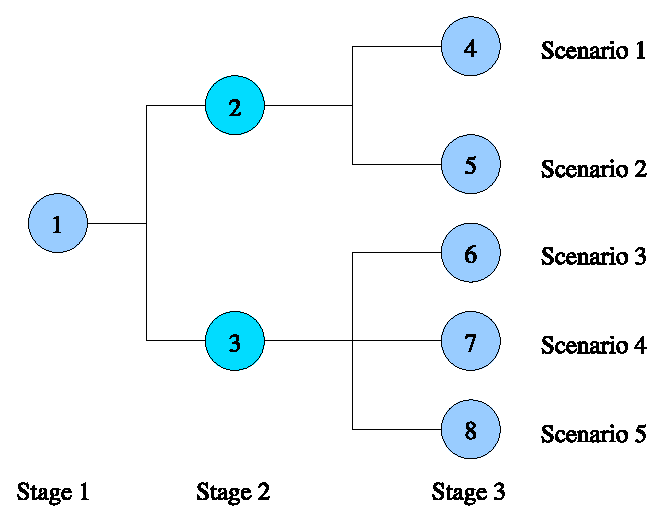
\includegraphics[scale=0.6]{figures/tree.eps}
    \caption{Event tree.}
    \label{fig:EventTree}
  \end{center}
  \vspace{-3ex}
\end{figure}

To each node of the event tree we associate a set of constraints, an 
objective function, and the conditional probability of visiting the 
node from its parent node in the previous stage.
The probability of each scenario is the product of the 
conditional probabilities of visiting each node on the path.

It should be noted that usually a very large number of scenarios is
needed to adequately capture the characteristics of the underlying
continuous distribution, particularly in the multi-stage setting.
In this case, the number of scenarios grows exponentially with the
number of decisions considered at each stage.
The size of the scenario tree determines the size of the optimization
program.

The question of how to generate an appropriate scenario tree
is not trivial, and has received extensive attention in the
literature 
\cite{DupacovaConsigliWallace,HoylandKautWallace,HoylandWallace,Pflug01}.

%
%
\subsection{The deterministic equivalent formulation}
\label{DetEqForm}

A natural formulation of a stochastic programming problem relies on 
recursion to describe the dynamics of the modelled process.
The term {\it recourse} means that, at each stage, the decision 
variables adapt to the different outcomes of the random parameters.
For ease of presentation, we consider the linear version of the
recourse problem:
%
\be \label{eq:SLPRecourse}
\begin{array}{rl}
  \min & c^T x + \E_\xi[\min\, q(\xi)^T y(\xi)]     \\
  \text{s.t.} &  Ax                       = b,      \\
	      &  T(\xi) x + W(\xi) y(\xi) = h(\xi), \\
	      &  x \geq 0,\; y(\xi) \ge 0,
\end{array}
\ee
%
where $y(\xi)$ denotes the recourse action which depends on the 
outcome of the random process $\xi$. 
Note that (\ref{eq:SLPRecourse}) combines in a single formulation
both (\ref{eq:SP1}) and (\ref{eq:SP2}).
After discretizing $\xi$ 
according to $P(x^i=\xi_i) = p^i$, and using the notation 
$T^i = T(\xi_i)$ (and analogously for $h^i$, $W^i$, $y^i$ and $q^i$), 
problem (\ref{eq:SLPRecourse}) can be written in the 
{\em deterministic equivalent formulation}:
\be \label{eq:DetEq-2stage}
\begin{array}{rlllll}
\min & c^T x + \sum_i p^i(q^i)^T y^i \\
\mbox{s.t.} & Ax              &        &          & = b,   \\
            & T^1 x + W^1 y^1 &        &          & = h^1  \\
	    & \quad\vdots     & \hspace{-1em}\ddots & & \;\vdots \\
            & T^n x           &        &+\; W^n y^n & = h^n \\
            & x \geq 0,\; y^i \ge 0.
\end{array}
\ee
The deterministic equivalent formulation is derived by writing
explicitly each possible realisation of the random parameters.
The formulation (\ref{eq:DetEq-2stage}) does not have any stochasticity
left, but is completely deterministic, and is therefore a common
linear programming problem of (very) large dimensions.
Also note that problem (\ref{eq:DetEq-2stage}) displays a
dual-block angular structure
in the constraint matrix.

\fb{
Make a step from two-stage to multistage.
}

To formulate the deterministic equivalent of the multi-stage 
stochastic programming problem we first need to enumerate all nodes 
of the event tree. We use a breadth-first 
search order, i.e., we start from a root node corresponding 
to the initial stage and end with leaf nodes corresponding 
to the last stage. In this case, the constraint matrix displays
a nested dual-block angular structure.

Let $t = 1,2,\ldots,T$ denote the stage and let $\mathcal{L}_t$ 
be the set of nodes at stage $t$.
With $a(l)$ we denote the direct ancestor of node $l\in\mathcal{L}_t$ 
(which is a node that belongs to stage $t-1$), and with
$\mathcal{D}_l\subset\mathcal{L}_{t+1}$ the set of children of node $l$.
The decision variables are superscripted with the node number $l$;
similar notation is used for the corresponding matrix and vector blocks.
The total number of scenarios is $N$.

The main constraint that describes the dynamics of the system has the form 
\[
  T^{l}x^{a(l)} +W^{l}x^{l} =h^{l}, \qquad l \in\mathcal{L}_t, t=2,\ldots,T,
\]
%
where $T^{l}$ is the technology matrix that varies 
with the node in the event tree, and $W^{l}$ is the recourse
matrix that, in general, depends on realisations within the same stage,
but often varies only with time.

The deterministic equivalent formulation of the multi-stage 
problem has the following general form:
\begin{equation}  \label{DetEquiv}
  \begin{array}{rrcll}
  \min & \displaystyle\sum_{t=1}^T\sum_{l\in\mathcal{L}_t} p^l (q^l)^T x^{l}\\
  \mbox{s.t.} & W^{l_1} x^{l_1} &\!\!\!\! = h^{l_1}, 
                               &\; l_1\in\mathcal{L}_1 \\
    & T^{l_t} x^{a(l_t)} + W^{l_t} x^{l_t} &\!\!\!\! = h^{l_t}, 
                               &\; l_t\in\mathcal{L}_t,\; t = 1,\dots,T, \\
    & x^{l_t} &\!\!\!\!\!\!\! \geq 0,
                               &\; l_t\in\mathcal{L}_t,\; t = 1,\dots,T. \\
  \end{array}
\end{equation}

Note that the probabilities in the objective function of problem 
(\ref{DetEquiv}) are the unconditional path probabilities: $p^l$ is 
the probability that a path goes through node $l$, which equals the 
product of the conditional probabilities along the path from the root 
to the node $l$.

If the event tree is traversed with depth-first-search ordering of the 
nodes during the generation of the mathematical program, the 
corresponding constraint matrix displays a nested dual block-angular 
structure.
Figure~\ref{fig:deteq} displays the two possible structures 
for the event tree of Figure~\ref{fig:EventTree} according 
to the chosen ordering of nodes.
%
\begin{figure}[ht]
  \centering
    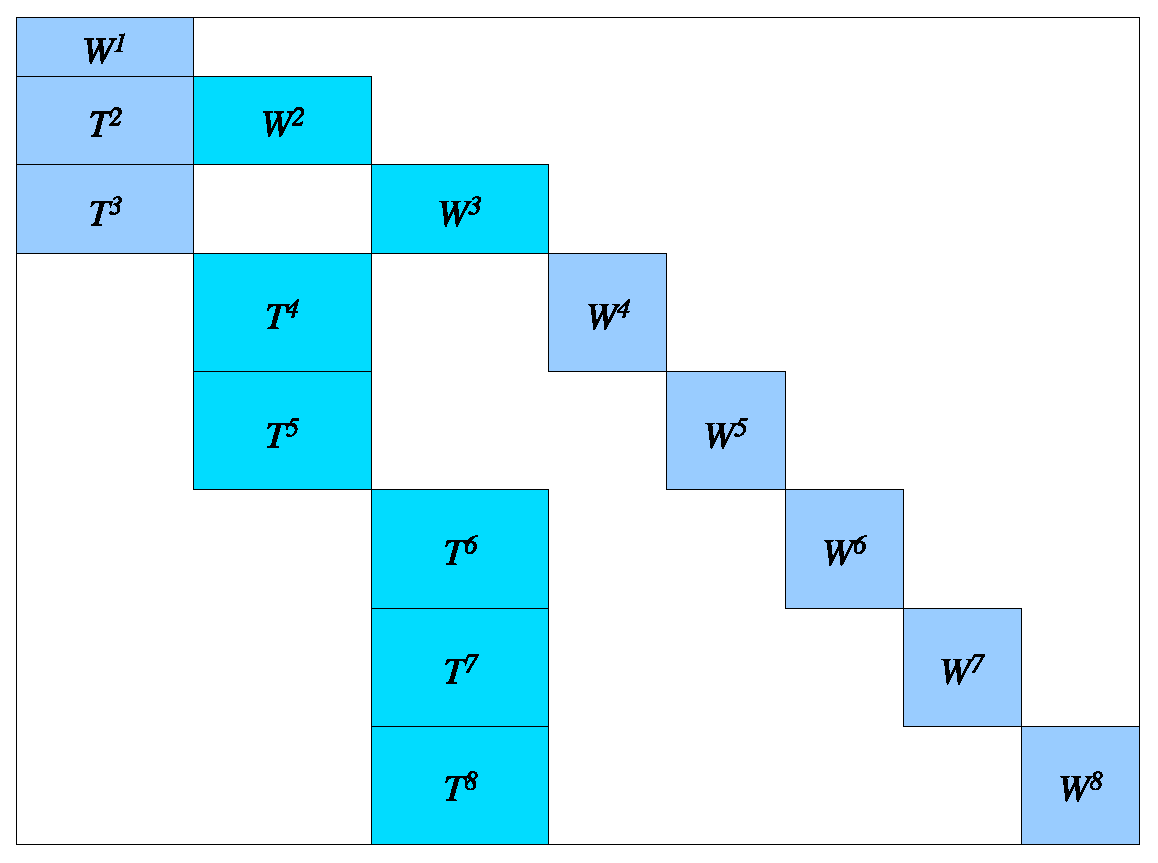
\includegraphics[scale=0.37]{figures/deteq-bfs.eps} \hfill
    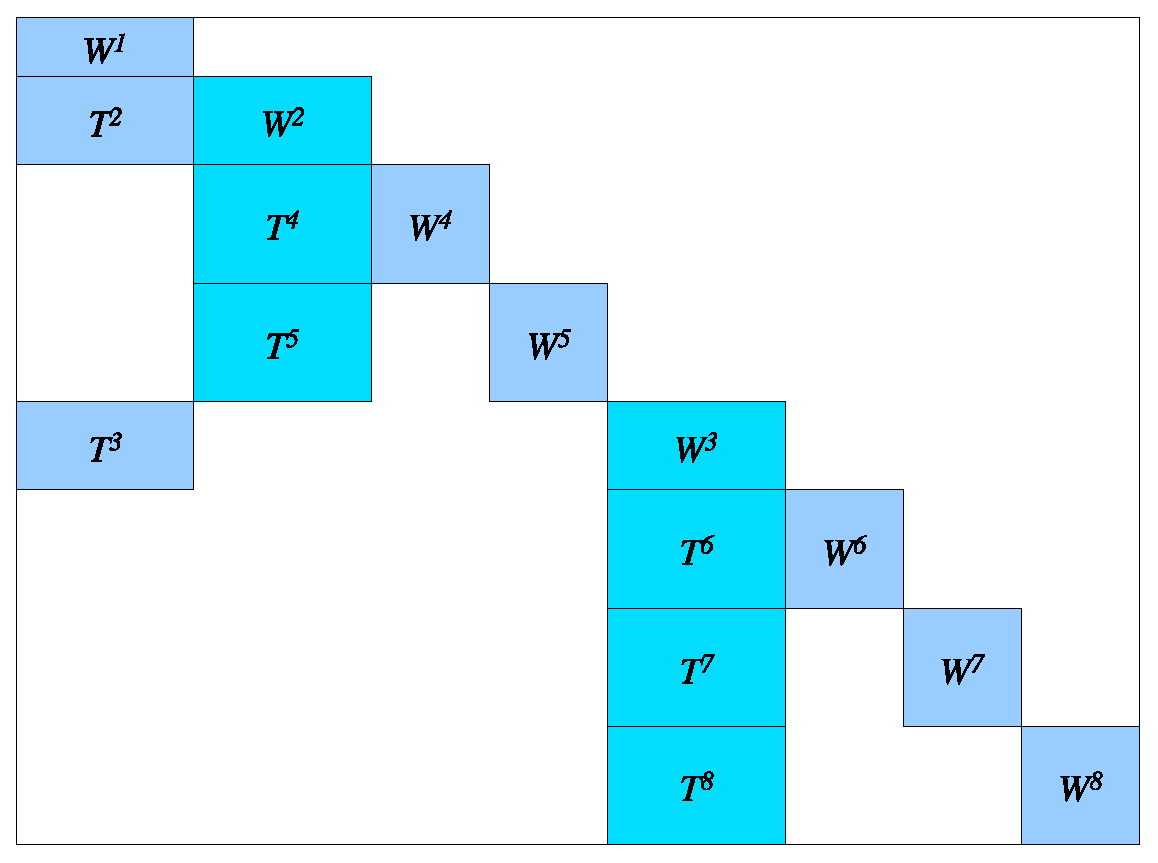
\includegraphics[scale=0.37]{figures/deteq-dfs.eps}
    \caption{Deterministic equivalent corresponding to the event tree 
             of Figure~\ref{fig:EventTree}, with nodes listed in breadth-first 
             order (left) and depth-first order (right).}
    \label{fig:deteq}
\end{figure}
%
While the different ordering of blocks whithin the matrix is not 
relevant for general-purpose solvers, the
structure-exploiting software \OOPS \cite{GondzioSarkissian} can take 
full advantage of the nested dual-block angular structure resulting
from the depth-first ordering in its internal object-oriented
linear algebra representation.

Clearly, (\ref{DetEquiv}) represents a structured linear program. Its 
structure should be exploited in the solution algorithm.
Several solution methods for stochastic linear programs have been 
presented in the literature. These often rely on some decomposition
approach \cite{Birge85,LinderothWright03,MulveyRuszczynski}, among others.
Kall and Mayer \cite{KallMayer} provided a comparison of different
solution algorithms for stochastic linear programming problems.
In what follows, instead, we consider solving the deterministic equivalent
problem directly through an interior point method.


%
% Section
%
\section{A reduced-tree warm-start iterate}
\label{sec:ReducedTree}

We already surveyed warm-start strategies in Section~\ref{sec:WarmStart}.
While those strategies apply to
general linear problems, we introduce an approach tailored to
stochastic programming. In particular, we propose to exploit the structure
inherent to a stochastic programming problem to generate a good 
warm-start iterate.

In the event tree corresponding to a large multistage program, 
the numerous leaf nodes descend from a relatively small number of 
branches in the first few stages. Two ``neighbouring'' scenarios, 
that is two scenarios that have common nodes, may display large 
differences concerning later stage decisions, but the decisions 
taken in the earlier stages are identical (nonanticipativity).
Moreover, there may be very little difference among 
scenarios, and so the large-scale problem can provide a fine-grained 
solution to a problem that could have been solved more coarsely by 
using a much smaller tree. 

These observations suggests a
warm-start technique that can be applied in the context of interior 
point methods. A warm-start solution is obtained by solving the 
stochastic optimization problem for a reduced event tree, whose 
dimension is much smaller than that of the complete one. The solution 
to the reduced problem is used to construct an advanced iterate for 
the complete formulation. We provide evidence that this novel way 
of exploiting the problem structure to generate an initial point 
provides a better iterate (in terms of centrality, feasibility, 
and closeness to optimality) than the one produced by a generic 
strategy.

Techniques for reducing the size of the scenario tree have been studied 
before from a probabilistic perspective; in some cases considerable 
savings can be obtained with such methods. Among others, 
Dupa\v{c}ov{\'a} \etal \cite{Dupacova} discuss an optimal scenario 
reduction technique that couples a large reduction of the scenario 
tree with a small loss in accuracy. In their example, a reduction by 
50\% of the scenario tree still maintains about 90\% of the original 
accuracy.
In this paper, we are interested in capturing some aspects of the 
stochasticity of the event tree without assuming further knowledge on 
the underlying stochastic process that generated it. Given this difference 
from what is required for example by \cite{Dupacova}, we will use less 
sophisticated arguments in finding a reduced tree.
We remark that if we have knowledge of the underlying stochastic process,
then we could exploit it in the generation of the reduced tree.

We first study how to build a reduced tree by choosing just 
some of the possible scenarios. We provide some insight on how to make 
this selection, so that our choice performs better than an arbitrary 
one.
Then we discuss how to obtain a warm-start solution from the reduced 
tree that corresponds to the chosen scenarios.
Our aim is to generate a warm-start iterate that allows to solve to 
optimality the complete problem in fewer iterations (and less computing 
time) than by a standard starting point heuristic \cite{Mehrotra92}.
With these aims, we propose a way of choosing a subset of scenarios 
that we believe to be sufficiently representative of the whole tree.
The algorithm can be summarised in the steps of
Algorithm~\ref{alg:OverallAlgorithm}.
%
\begin{algorithm}[h]
  \caption{Reduced-tree warm-start algorithm}
  \begin{algorithmic}[0]  \label{alg:OverallAlgorithm}
    \REQUIRE The complete event tree $\Ctree$.
    \smallskip
    \STATE Generate a reduced event tree $\Rtree\subset\Ctree$;
    \smallskip
    \STATE Solve the corresponding deterministic equivalent with a loose 
           tolerance;
    \smallskip
    \STATE Use this solution to construct a warm-start iterate for the 
    complete problem;
    \smallskip
    \STATE Solve the complete problem to optimality.
  \end{algorithmic}
\end{algorithm}

In the rest of this section we define our method of generating a 
reduced tree and describe the construction of the complete warm-start 
iterate.

%
%
\subsection{Scenario distance}
\label{sec:ScenarioDistance}

For the purposes of generating a reduced scenario tree (see
Section~\ref{sec:ReducedTreeGeneration}), we need to define a measure 
of distance between scenarios.
Recalling that a scenario is a path in the event tree from the root to 
a leaf node, we can encode a scenario $s_k$, $k = 1, \ldots, N$, as an 
ordered set of nodes $s_k = \{ l_1, \ldots, l_T : \: l_t = a(l_{t+1}), \:
t=1,\ldots, T-1 \}$.
To each node $l_t$ of the tree we associate the tuple 
$\eta^{l_t} = \{ T^{l_t}, W^{l_t}, h^{l_t}, q^{l_t} \}$ of matrices, 
right-hand side and objective coefficients.

We first define the distance between two nodes $i_t$ and $j_t$ that 
belong to the same stage $t$ as
%
\be \label{eq:Distance}
   d(\eta^{i_t}, \eta^{j_t}) = \| T^{i_t} - T^{j_t} \| + \| W^{i_t} - W^{j_t} 
   \| + \| h^{i_t} - h^{j_t} \| + \| q^{i_t} - q^{j_t} \|,
\ee
%
for some norm $\| \cdot \|$.
%
Hence, we define the distance between scenarios $i$ and $j$ as
\[
  D(s_i, s_j) = \sum_{t=1}^T d(\eta^{i_t}, \eta^{j_t}),
                \quad i_t \in s_i, j_t \in s_j.
\]

Therefore, scenarios that belong to the same branch of the tree will 
have smaller distance in general, as they share some of the nodes. 
Conversely, scenarios are likely to be farther away if they do
not share nodes apart from the root.

%
%
\subsection{Reduced tree generation}
\label{sec:ReducedTreeGeneration}

We generate the reduced tree by taking into account both 
the structural and the stochastic information available from the 
problem formulation. By structural information we mean the shape of 
the event tree, i.e. how the tree branches at the various stages; by 
stochastic information we refer to the probabilities associated to 
each node in the tree, and consequently to each scenario. Hence we 
adopt two complementary strategies. First we choose a subset of 
branches of the event tree; then, in each branch, we choose the most 
representative leaf nodes.

We try to capture the structure of the complete tree by making sure 
that a sufficient number of different early stage decisions will 
appear in the reduced tree. In some sense, we look for a way to span 
the breadth of the complete tree. For a defined small value $k < T$, where 
$T$ is the number of stages in the problem, we choose some of the 
nodes at the $k$-th stage, together with all their ancestors up to the 
root, to appear in the subtree. The choice on the nodes to appear in
the reduced tree should be guided by probabilities.
The rationale for this strategy is to ensure that our warm-start 
iterate has a good representation of the decisions to be taken 
in the first few stages, as getting early decisions right is fundamental
for an easier optimization of the later stages.
%
To illustrate this idea, suppose we deal with a multistage setting where 
there are $T=4$ stages, such as in the tree of Figure~\ref{fig:Tree}: 
for $k=2$ we choose nodes 1, 2 and 3 to be in the reduced tree.
\begin{figure}[ht]
  \begin{center}
    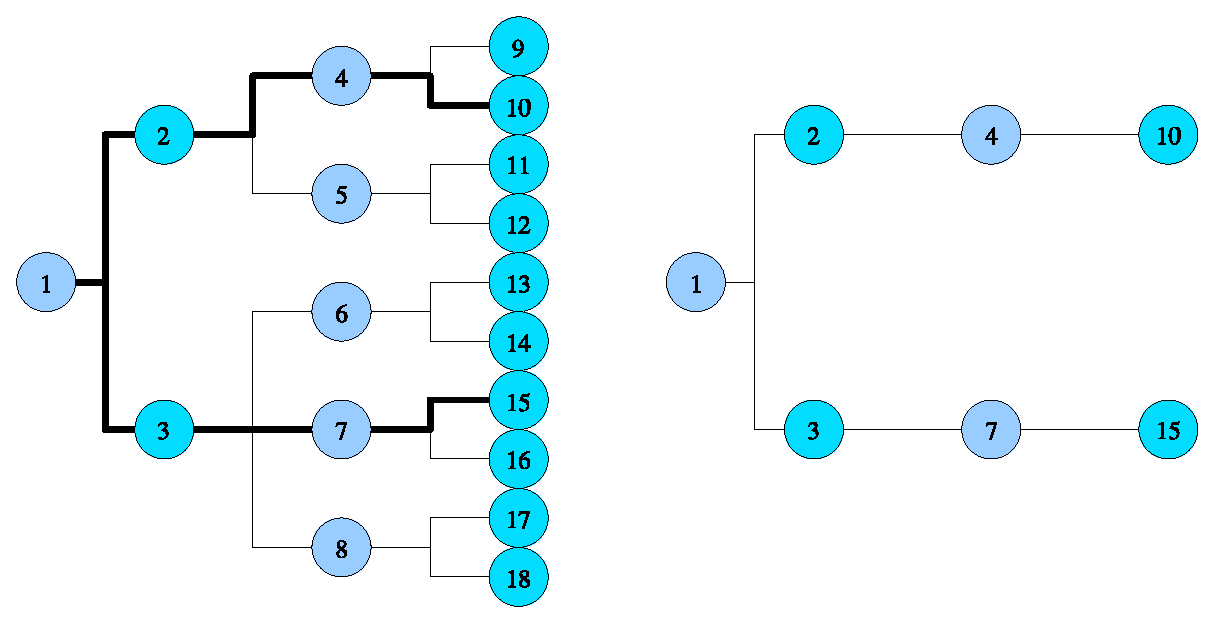
\includegraphics[scale=.6]{figures/redtree.eps}
    \caption{Complete tree and the reduced tree corresponding to the
             chosen scenarios (in bold).}
    \label{fig:Tree}
  \end{center}
  \vspace{-3ex}
\end{figure}

Each of the chosen nodes in the $k$-th stage now becomes the root of a 
branch of the tree, which we call a subtree. In each subtree we choose 
the scenario that minimises the distance to an average scenario in the 
same subtree.
%
Let $S_t$ be the set of nodes in the subtree $S$ at stage $t$, and 
$|S_t|$ its cardinality. For each stage $t$ within subtree $S$, 
we determine an artificial node $n_t$ by averaging the data 
associated to all nodes at this stage:
\[
n_t = \frac{1}{|S_t|} \sum_{l_t \in S_t} (T^{l_t}, W^{l_t}, h^{l_t}, q^{l_t}),
\quad k < t \le T.
\]

We define the average scenario for subtree $S$ as the ordered
set of nodes $s_k = \{ l_k, n_{k+1}, \ldots, n_T \}$.
Therefore, the average scenario $\bar s$ (in the complete tree) 
is obtained by listing the 
nodes from the root of the tree to the root of the subtree $S$, and 
then by appending the average nodes. We define it as
\[
\bar s = \{\, l_1, \ldots, l_k, n_{k+1}, \ldots, n_T \,\},
\]
where $l_t = a(l_{t+1})$ for $t = 1,\ldots, k-1$.
Scenario $\bar{s}$ is completely artificial, and there is no guarantee 
that it is feasible: therefore we cannot use it directly as our 
representative scenario. Instead, we use it as a reference point to 
which compare all other scenarios, and thus find the closest scenario 
among the existing ones: this way we do not introduce spurious 
infeasibilities. Hence, in the subtree $S$ we choose the 
representative scenario $s^*$ as 
%
\be  \label{repScenario}
   s^* = s_k, \quad k = \arg\min_{i\in S} \{ (1-p^i) D(s_i, \bar{s}) \},
\ee
%
where, since our ultimate goal is to find the most representative scenario in 
the subtree, we use the term $(1-p^i)$ to ``bring closer'' scenarios 
that have a higher probability of occurring.

The reduced tree selection induces a function $r: \Ctree \to \Rtree$ 
that maps each node of the complete tree to a corresponding node 
in the reduced tree in the following way: if $i \in \Rtree$, then
$r(i) = i$; if $i\not\in \Rtree$, then we choose as $r(i)$ the node in 
the representative scenario corresponding to node $i$ belonging to the
same stage $t$ as node $i$. In other words, to get from node
$i\in\Ctree$ to $r(i)\in\Rtree$ we walk up the tree $\Ctree$ until we
find a node that is also in $\Rtree$ and from there walk back down
the reduced tree until we arrive at the same stage as the original node

This mapping is used to decide how to initialise 
the warm-start iterate for the complete tree, as presented in the
next section. We remark that our generation process guarantees
that for each $i \in \Ctree$, the following properties hold:
\be  \label{eq:ReducedTreeProperties}
  a(r(i)) \in \Rtree, \quad \mbox{ and } \quad a(r(i)) = r(a(i)),
\ee
that is if a node is in the reduced tree so is its parent, and the
mapping $r(.)$ preserves the parent-child relationship. We will also
need the sets 
$\mathcal{I}_k = \{\, i \in \Ctree : r(i) = k \,\}$, $k \in \Rtree$,
the set of nodes in the complete tree that are initialised by a given
node $k\in\Rtree$.

Continuing the example started above, we consider two subsets of 
scenarios, corresponding to nodes 9--12 (for the subtree rooted at 
node 2) and to nodes 13--18 (for the subtree rooted at node 3). Within 
each subset we build the scenario of average nodes and then find the 
representative scenario.
The resulting reduced tree is shown in the right of Figure~\ref{fig:Tree}.

It should be noted that the reduced tree generation process can be
interpreted as a node-aggregation process: all nodes in
$\mathcal{I}_k\subset\Ctree$ are aggregated into a single node $k\in\Rtree$.
The node-aggregation implies the node probabilities $p_R^k$ associated
with each node $k\in\Rtree$; we use:
 \be  \label{eq:UpdatePathProbs}
  p^l_R = \sum_{i \in \mathcal{I}_l} p^i.
 \ee
Here and in the following we use the notation that symbols referring
to the reduced tree (such as $\Rtree$, $p_R^i$) carry the subscript
$_R$ to distiguish them from the same symbols used for the complete tree.
As will be seen later it is advantageous if the aggregation of nodes
is balanced throughout the tree. On average every node in the reduced
tree corresponds to $|\Ctree|/|\Rtree|=n/n_R$ nodes in the full tree, so for
a totally balanced aggregation we would expect 
\[
  \frac{p^i}{p_R^{r(i)}}\frac{n}{n_R}\approx 1.
\]
We denote by $\rho$ the deviation from this
\be  \label{eq:rho}
  \rho := \max_{i\in\Rtree}\max\left\{\frac{p^i}{p_R^{r(i)}}\frac{n}{n_R}, 
                                 \frac{p_R^{r(i)}}{p^i}\frac{n_R}{n}\right\}.
\ee

It is worth noting the effect of the probabilities update
(\ref{eq:UpdatePathProbs}) on the conditional path
probabilities. Denote by $\delta^i := p_i/p_{a(i)}$ the probability of
reaching node $i$, given that its parent $a(i)$ has already been
reached and similarly for $\delta^i_R$. For a node $l$ in the $k$-th
stage where the subtree selection takes place we have (by dividing
(\ref{eq:UpdatePathProbs}) through by $p_{a(l)}$ and since 
$a(l)\in \Rtree\subseteq\Ctree$)
\[
  \delta_R^l = \sum_{i \in \mathcal{I}_l} \delta^i
\]
for a node $l$ below stage $k$ we have $\delta_R^l=1$ (since there is
only one, the representative, scenario in each subtree). 
%This is
%however also equal to the sum of the conditional probabilities of the
%children of node $l$, so that we have
In either case we can write
\be  \label{eq:UpdateCondProbs}
\delta_R^l = \sum_{i \in \mathcal{I}_l\cap D_{a(l)}} \delta^i.
\ee

%
%
\subsection{Construction of the warm-start iterate}
\label{sec:Construction}

Consider the linear programming problem in standard form
\be  \label{eq:CompleteProblem}
\min\;  c^T x \;\quad \mbox{s.t. }\; Ax = b, \;\; x \ge 0,
\ee
where $A \in \R^{m \times n}$ is full rank, 
$x, c \in \R^{n}$ and $b \in \R^{m}$. 
Problem (\ref{eq:CompleteProblem})
corresponds to the deterministic equivalent \eqref{DetEquiv} generated from a
given event tree $\Ctree$. We will refer to it as the 
{\em complete problem}.

From the reduced tree, which we denote by $\Rtree$, 
we build the reduced deterministic 
equivalent problem
\be \label{eq:ReducedProblem}
\min\; c_R^T x_R \;\quad \mbox{s.t. }\; A_R x_R = b_R, \; x_R \ge 0,
\ee
with $A_R \in \R^{m_R\times n_R}$, $x_R \in 
\R^{n_R}$ and $b_R \in \R^{m_R}$. This problem is 
much smaller than the complete formulation, and hence we expect it to 
be much easier to solve.
We call problem \eqref{eq:ReducedProblem} the {\em reduced problem}.

We solve problem (\ref{eq:ReducedProblem}) with an interior point method. 
For the reasons presented in Section~\ref{sec:WarmStart}, we do not 
aim for optimality, but instead we aim for a sufficiently advanced 
primal--dual feasible point, i.e. we seek a
$(x_R^*,y_R^*,s_R^*)\in\mathcal{N}_s(\gamma)$ corresponding to a
sufficiently advanced barrier parameter $\mu^*_R$.

This iterate is used to construct the warm-start iterate
$(\hat{x}, \hat{y}, \hat{s})$ for the
complete problem on a node-by-node basis. The sections of the vectors
$\hat{x}, \hat{y}, \hat{s}$ correspoding to node $i\in\Ctree$ are
initialised from the sections of the vectors 
$x_R^*,y_R^*,s_R^*$ correspoding to node $r(i)\in\Rtree$. This process
will be detailed below.

Denote by $\hat x^{i}, \hat y^{i}, \hat s^{i}$ the part of the vectors
$\hat{x}, \hat{y}, \hat{s}$ corresponding to node $i\in\Ctree$ and likewise
$x_R^{i}, y_R^{i},  s_R^{i}$ for components of the solution of the
reduced problem. Then we construct the starting point for the complete
problem in the following manner:
\be  \label{eq:WarmstartSolution}
  \hat x^{i} = x_R^{r(i)}, \qquad 
 (\hat y^{i}, \hat s^{i}) = \frac{p^{i}}{p_R^{r(i)}} (y_R^{r(i)}, s_R^{r(i)}),
  \qquad\forall i \in \Ctree,
\ee
where $p^i_R$ is computed according to (\ref{eq:UpdatePathProbs}).
This means that the dual reduced-tree solution is spread among the
nodes it initialises, as can be seen here:
\[
   \sum_{i \in \mathcal{I}_k} (\hat y^i, \hat s^i)
  = \sum_{i \in \mathcal{I}_k} \frac{p^i}{p^k_R} (y^k_R, s^k_R)
  = (y^k_R, s^k_R) \frac{1}{p^k_R} \sum_{i \in \mathcal{I}_k} p^i 
  = (y^k_R, s^k_R), \qquad\forall k \in \Rtree.
\]

Considering again the example of Figure~\ref{fig:Tree}, suppose that 
in the reduced tree we accepted only the scenarios that end at 
node 10 and node 15, so that the reduced tree consists of nodes 
1, 2, 3, 4, 7, 10 and 15. By solving the corresponding reduced problem, 
we obtain the parts of the solution vector associated to such 
nodes: these can be used directly in the complete iterate
(Figure~\ref{fig:Solution} top). 
We fill the missing elements 
by reproducing the solution from the nodes in the same subtree 
and the same stage (Figure~\ref{fig:Solution} bottom).
The proposed way of constructing the complete iterate is easy to
implement and its execution time is negligible.
%
\begin{figure}[ht]
  \begin{center}
    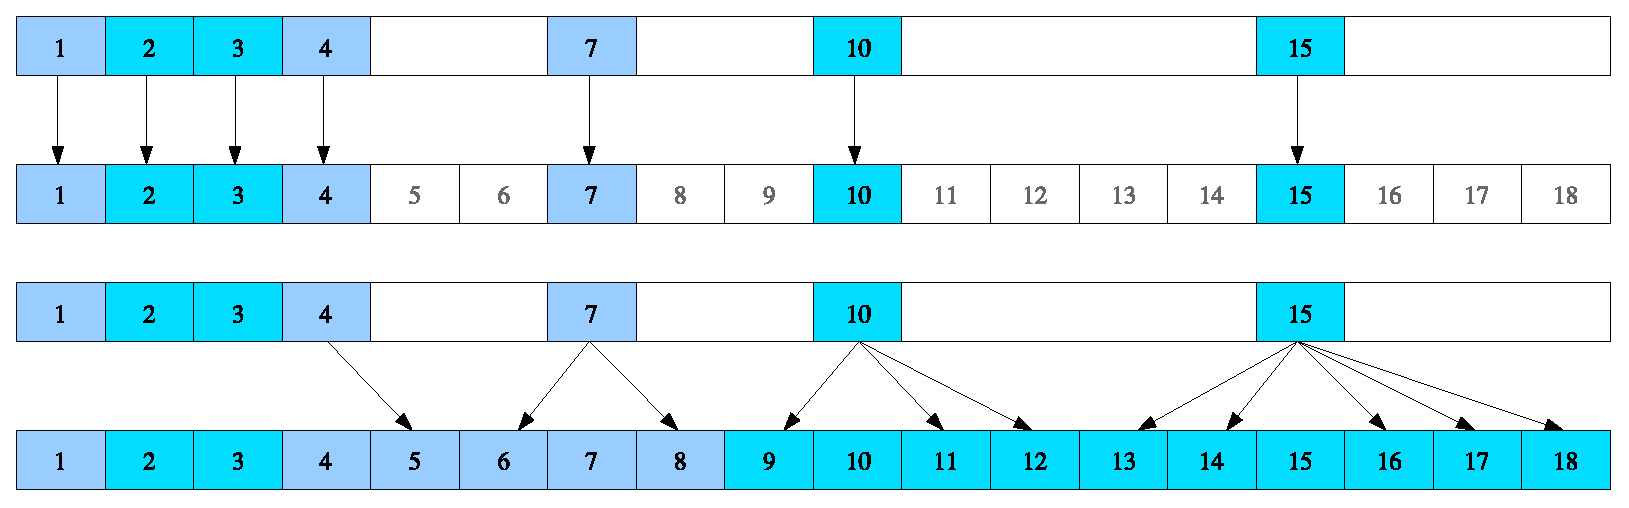
\includegraphics[scale=.51]{figures/solution.eps}
    \caption{Generation of the warm-start iterate.}
    \label{fig:Solution}
  \end{center}
  \vspace{-3ex}
\end{figure}

\ignore{
This simple strategies can be further 
generalised by considering a linear combination of the solutions 
corresponding to nodes that belong to the same stage. In this sense, 
the parts of the solution for nodes 4 and 7 may be used to initialise 
the solution for nodes 5, 6 and 8 (similarly for nodes 10 and 15 to 
initialise the starting solution for the other leaf nodes).
}

%
% Section
%
\section{Analysis of the warm-start iterate}
\label{sec:Analysis}

In this section we study how the warm-start iterate generated with 
the procedures presented above satisfies the conditions expressed by 
Gondzio and Grothey \cite{GondzioGrothey03}. 
Contrary to what is assumed in both \cite{YildirimWright} and 
\cite{GondzioGrothey03}, in our approach the dimension of the problem changes, 
as the reduced tree problem is, by construction, much smaller than the 
complete problem.

However, in a similar way as we did with the solution vector, 
we can expand the reduced problem to one which has the same dimension 
as the complete problem (\ref{eq:CompleteProblem}) by replicating
the blocks in the coefficient matrix and in the objective and right-hand 
side vectors, as shown in Figure~\ref{fig:ExpandedSystem}.
%
\begin{figure}[ht]
  \begin{center}
    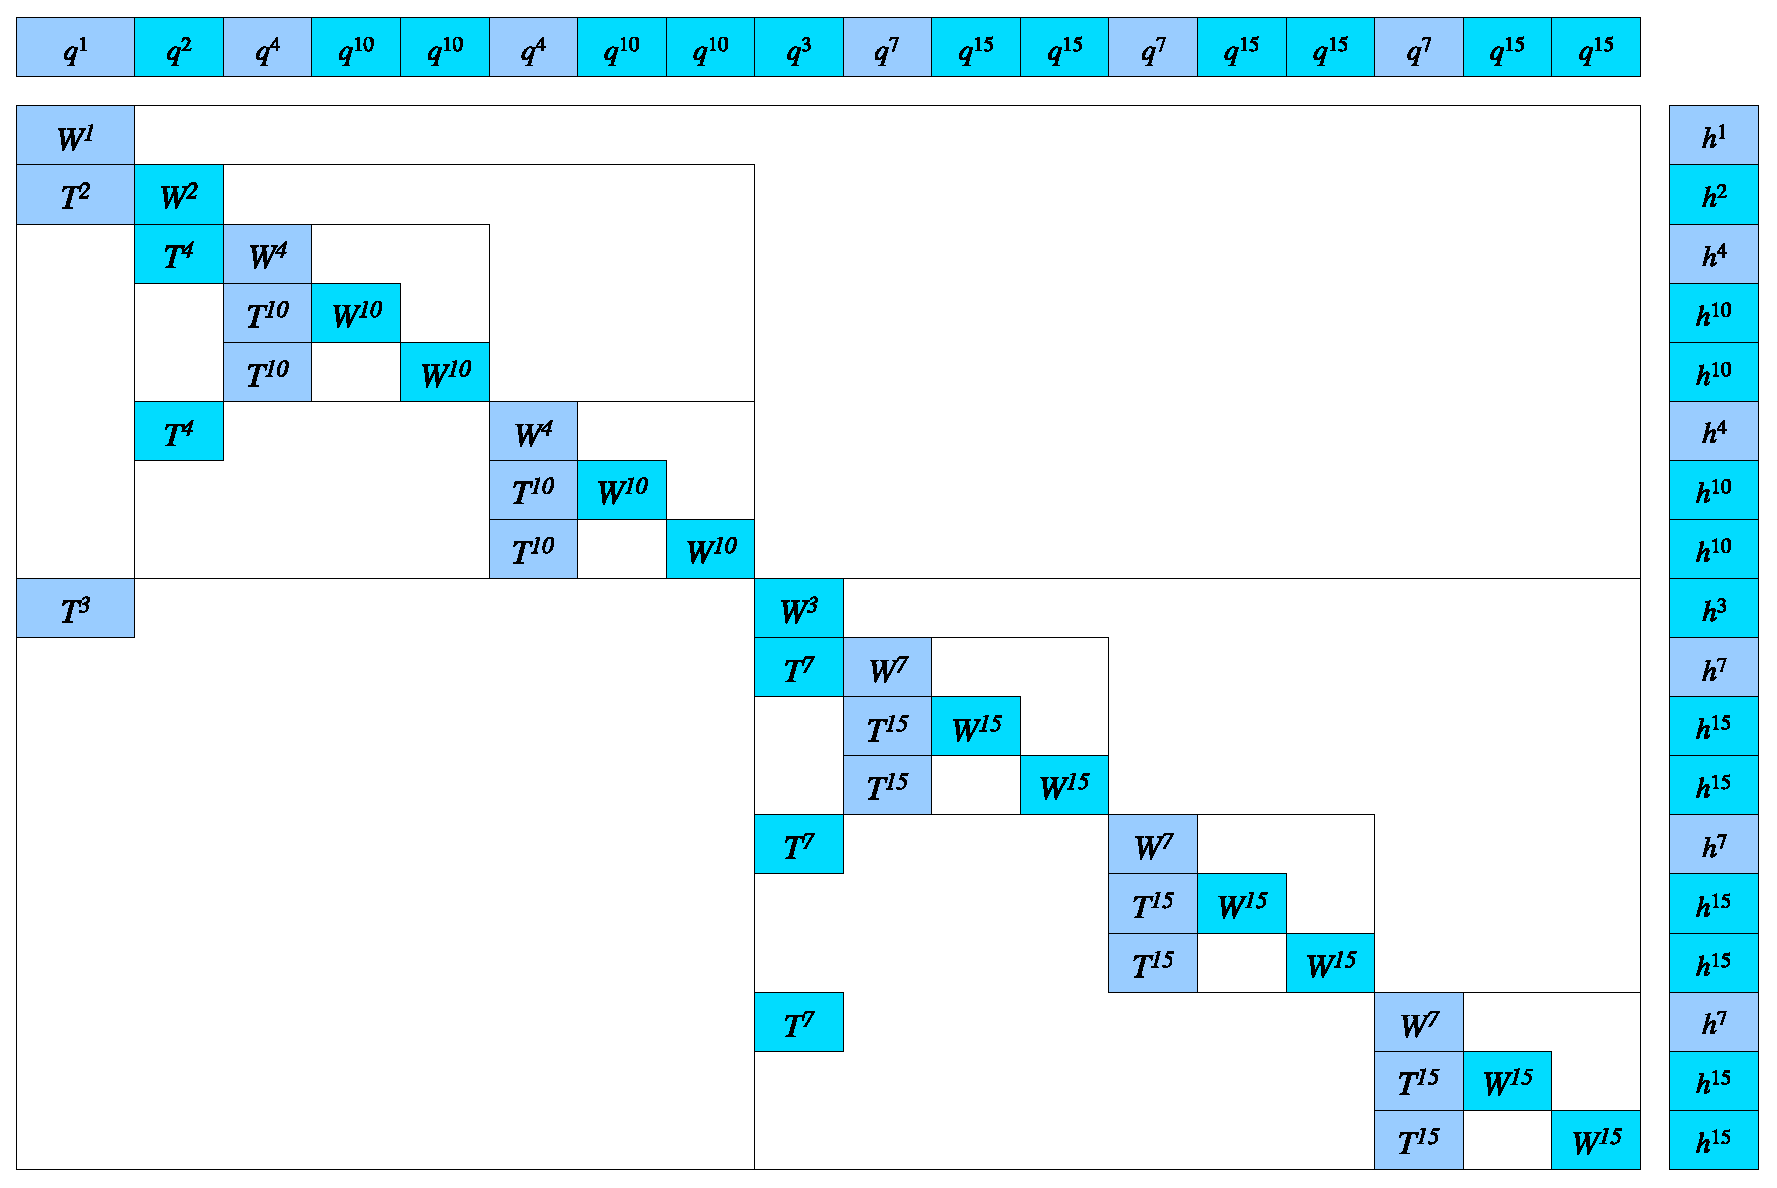
\includegraphics[scale=.50]{figures/expandedsystem.eps}
    \caption{The expanded system for the event tree of Figure~\ref{fig:Tree}.}
    \label{fig:ExpandedSystem}
  \end{center}
  \vspace{-3ex}
\end{figure}

This corresponds to creating the (artificial) expanded problem
\be \label{eq:ExpandedProblem}
\min\; \hat{c}^T x \;\quad \mbox{s.t. }\; \hat{A} x = \hat{b},
    \; x \ge 0,
\ee
the dimension of which, $\hat{A} \in \R^{m\times n}$, 
$\hat{c}, x \in \R^{n}$ and $\hat{b} \in \R^{m}$,
corresponds to the dimension of the complete problem 
(\ref{eq:CompleteProblem}).
Using the notation introduced earlier, we will denote 
all symbols referring to the expanded problem with a hat $\hat{\cdot}$.

To analyse the warm-start iterate we can now follow a two-step
procedure. First we note that from an advanced iterate 
$(x_R, y_R,  s_R)\in\mathcal{N}_{R,s}(\gamma)$ for the reduced
problem the procedure in (\ref{eq:WarmstartSolution}) constructs a
primal--dual feasible point $(\hat{x}, \hat{y}, \hat{s})$ for the {\em
expanded} problem. Indeed we will show 
$(\hat{x}, \hat{y}, \hat{s})\in\hat{\mathcal{N}}_s(\hat{\gamma})$
in Theorem~\ref{th:FeasibleExpandedSolution}. In the second step we
can use this iterate to warmstart the complete problem. Since in the
step from the expanded to the complete problem only the problem data
but not its size changes, the methods developed in
\cite{GondzioGrothey03,YildirimWright} can be used to analyse the 
warm-start iterate.

We start the analysis with a technical result.

\begin{lemma}  \label{th:SumOfTerms}
Let $l\in\Ctree$, then
\[
\sum_{i \in \mathcal{D}_{l}} {T^{r(i)}}^T \hat y^i
  = \frac{p^{l}}{p^{r(l)}_R}\sum_{k \in \mathcal{D}_{r(l)}^R}
    {T^k}^T y^k_R.
\]
\end{lemma}
%
\begin{proof}
We have this chain of identities:
\[
\begin{split}
\sum_{i \in \mathcal{D}_{l}} {T^{r(i)}}^T \hat y^i
  &= \sum_{i\in\mathcal{D}_{l}} {T^{r(i)}}^T y^{r(i)}_R\frac{p^i}{p^{r(i)}_R}\\
  &= \frac{p^{l}}{p^{r(l)}_R}\sum_{i \in \mathcal{D}_{l}} {T^{r(i)}}^T
    y^{r(i)}_R \frac{\delta^i}{\delta_R^{r(i)}}\\
  &= \frac{p^{l}}{p^{r(l)}_R}\! \sum_{k \in \mathcal{D}_{r(l)}^R} \!\!
       \frac{{T^k}^T y^k_R}{\delta_R^k}
       \sum_{i \in \mathcal{I}_k \cap \mathcal{D}_{l}}\!\!\! \delta^{i},
\end{split}
\]
where the second equal sign follows from $p^i = p^l\delta^i$ and
$p_R^{r(i)} = p_R^{r(l)}\delta_R^{r(i)}$ which is true since $l=a(i)$
and due to (\ref{eq:ReducedTreeProperties}) also $r(l) = a(r(i))$. The
third equal sign follows from the fact that we can partition
$\mathcal{D}_l$ according to which nodes of the reduced tree are used
for initilisation:
\(
  \mathcal{D}_{l} = \bigcup_{k \in \mathcal{D}_{r(l)}^R}
     \mathcal{I}_{k} \cap \mathcal{D}_{l}.
\)
The claim then follows from (\ref{eq:UpdateCondProbs}).
\end{proof}

\begin{theorem}  \label{th:FeasibleExpandedSolution}
If $(x_R, y_R, s_R)$ is primal and dual feasible for
the reduced problem (\ref{eq:ReducedProblem}),
then the warm-start solution $(\hat{x}, \hat{y}, \hat{s})$
obtained from (\ref{eq:WarmstartSolution}) is 
primal and dual feasible for the expanded problem (\ref{eq:ExpandedProblem}).
\end{theorem}
%
\begin{proof}
As $\hat x^{l} = x^{r(l)}_R$, primal feasibility is trivially
satisfied:
\be  \label{eq:RedTreePrimalContribution}
   T^{r(l)}\hat x^{a(l)} + W^{r(l)} \hat x^{l} =  h^{r(l)}, 
      \quad l \in \Ctree.
\ee
%
Now we consider dual feasibility. 
By assumption, the reduced problem solution satisfies 
the dual constraints:
\[
  {W^{r(l)}}^T y^{r(l)}_R +\sum_{i \in \mathcal{D}^R_{r(l)}} {T^{r(i)}}^T
     y^{r(i)}_R + s^{r(l)}_R = p^{r(l)}_R q^{r(l)},
     \quad r(l) \in \Rtree.
\]
Multiplying both terms by $p^{l}/p^{r(l)}_R$ we obtain
\[
  \frac{p^{l}}{p^{r(l)}_R} \Big( {W^{r(l)}}^T y^{r(l)}_R
     +\sum_{i\in \mathcal{D}_{r(l)}^R} {T^{r(i)}}^T y^{r(i)}_R + s^{r(l)}_R
     \Big) = p^{l} q^{r(l)},
\]
which, according to (\ref{eq:WarmstartSolution}) and 
Lemma~\ref{th:SumOfTerms}, becomes
\be  \label{eq:RedTreeDualContribution}
  {W^{r(l)}}^T \hat y^{l}+\sum_{i\in\mathcal{D}_{l}}{T^{r(i)}}^T \hat y^i
   + \hat s^{l} = p^{l} q^{r(l)}, \quad l \in \Ctree,
\ee
so $(\hat y, \hat s)$ satisfies
the dual constraints in the expanded problem.
\end{proof}

%
%
\subsection{Absorbing perturbations}

We argue that the difference between the data of the expanded 
problem (\ref{eq:ExpandedProblem}) and that of the original (complete) 
problem (\ref{eq:CompleteProblem}) can be interpreted as a perturbation 
between two problem instances of identical dimension. 
Clearly the expanded system has merely a theoretical
interest, as we use it to evaluate the magnitude of the 
perturbation introduced, and we never generate it in practice.

We assume that a feasible long-step path-following algorithm based on
the symmetric neighbourhood $\Nhood_s(\gamma)$ 
is used to solve the warmstarted complete problem. 
Although the constructed warm-start iterate $(\hat{x}, \hat{y}, \hat{s})$ 
from (\ref{eq:WarmstartSolution}) is feasible in the expanded problem, 
it is not feasible in the complete problem. 
As in \cite{YildirimWright,GondzioGrothey03} we will derive
conditions that guarantee to absorb these infeasibilities with one
{\em modification step}. 
For this consider the following Newton system:
\be \label{eq:NewtonSystem2}
\left[ \begin{array}{ccc}
    A & 0 & 0 \\ 0 &A^T & I \\ \hat{S} & 0 & \hat{X}
  \end{array} \right]
\left[ \begin{array}{c}
    \Delta x \\ \Delta y \\ \Delta s
  \end{array} \right] = 
\left[ \begin{array}{c}
    \xi_b \\ \xi_c \\ 0
  \end{array} \right],
\ee
where $\xi_b = b - A\hat{x}, \xi_c = c - A^T\hat{y}+\hat{s}$ are the
infeasibilities incurred by using the expanded iterate $(\hat{x},
\hat{y}, \hat{s})$ to warmstart the complete problem. 
Such a modification is termed a {\em Newton step correction} in
\cite{YildirimWright} or an {\em Additional centering iteration}
in \cite{GondzioGrothey06}. 
Gondzio and Grothey \cite{GondzioGrothey03} analyse the
same system, but are concerned with absorbing primal and dual
infeasibility separately by splitting (\ref{eq:NewtonSystem2}) into
two separate directions.
We will give a more general result and apply it to the situation of
warm start for stochastic programming problems. To avoid overburdening
notation we will drop the claret $\hat{}$ from the warm-start vectors.
The last equation of (\ref{eq:NewtonSystem2}) implies
\[
 s_i\Delta x_i + x_i\Delta s_i = 0, \qquad i = 1, \ldots, n.
\]

After some straightforward manipulation following the arguments of 
\cite{GondzioGrothey03}, the Newton
direction (\ref{eq:NewtonSystem2}) can be expressed in terms 
of the primal and dual residuals $\xi_b$, $\xi_c$ as
%
\begin{eqnarray}  \label{eq:Directions}
  \Delta x & \hspace{-1ex} = \hspace{-1ex} & 
  (XS^{-1} \! A^T (AXS^{-1} \!\! A^T)^{-1} \! AXS^{-1} \!\!-\!\! XS^{-1} )\xi_c
  \! + \! XS^{-1} \! A^T (AXS^{-1} \! A^T)^{-1} \xi_b, \nonumber \\
  \Delta y & \hspace{-1ex} = \hspace{-1ex} & 
  (AXS^{-1} A^T)^{-1} (AXS^{-1} \xi_c + \xi_b),                  \\
  \Delta s & \hspace{-1ex} = \hspace{-1ex} & 
  (I - A^T (AXS^{-1} \! A^T)^{-1} AXS^{-1} )\xi_c 
  \! - \! A^T (AXS^{-1} \! A^T)^{-1} \xi_b.            \nonumber
\end{eqnarray}

We consider the matrix
\[
  Q = I - S^{-1} A^T (A X S^{-1} A^T)^{-1} A X,
\]
and restate Lemma~3.2 of \cite{GondzioGrothey03},
which provides a bound on the norm of $Q$, in terms of
the symmetric neighbourhood $N_s(\gamma)$.

\begin{lemma}  \label{th:BoundQ}
If $w \in \widehat{\Nhood}_s(\gamma)$, then $\|Q\|_2 \le 1/\gamma$.
\end{lemma}
%
\begin{proof}
For a point $w \in \widehat{\Nhood}_s(\gamma)$, 
the following inequalities hold:
\[
  (x_i s_i)^{-1/2} \le (\gamma\mu)^{-1/2},
  \quad \mbox{ and } \quad
  (x_i s_i)^{1/2} \le (\mu / \gamma)^{1/2}.
\]
With some manipulations, we can express matrix $Q$ as
\[
Q = X^{-1/2}S^{-1/2} \left[ I - X^{1/2}S^{-1/2}A^T(AXS^{-1}A^T)^{-1}AX^{1/2}S^{-1/2} \right] X^{1/2}S^{1/2},
\]
where the term in square brackets is an orthogonal projection on the null
space of $AX^{1/2}S^{-1/2}$, so its Euclidean norm is 1.
As desired, we obtain
\[
  \| Q \|_2 = \| X^{-1/2}S^{-1/2} \|_2 \| X^{1/2}S^{1/2} \|_2 \le 1/\gamma.
  \qedhere
\]
\end{proof}

In the next Lemma we state sufficient conditions for the perturbations
to guarantee a full Newton step.

\begin{lemma}  \label{th:FullNewtonStep}
Let $w \in \widehat{\Nhood}_s(\gamma)$ be the warm-start iterate 
and define the scaled residuals 
\be  \label{eq:ScaledResiduals}
  \tilde \xi_b = X^{-1} A^T (A A^T)^{-1} \xi_b 
  \quad \mbox{ and } \quad 
  \tilde \xi_c = S^{-1} \xi_c.
\ee
If for $\beta < 1$ we have
\[
\|\tilde{\xi}_b\|_\infty + \|\tilde{\xi}_c\|_\infty 
    \le \beta\left(1 + \sqrt{n} / \gamma \right)^{-1},
\]
then the full Newton step (\ref{eq:NewtonSystem2}) from 
the warm-start iterate can be taken and absorbs the complete infeasibilities.
\end{lemma}
%
\begin{proof}
Using the definitions of the matrix $Q$ and of the relative residual 
vectors (\ref{eq:ScaledResiduals}),
the relations (\ref{eq:Directions}) simplify to
\[
   X^{-1}\Delta x = -Q \tilde{\xi}_c + (I-Q) \tilde{\xi}_b = -S^{-1}\Delta s,
\]
%\begin{eqnarray*}
%   X^{-1}\Delta x & \!\! = \!\! & 
%       -Q \tilde{\xi}_c + (I-Q) \tilde{\xi}_b, \\
%   S^{-1}\Delta s & \!\! = \!\! & 
%        Q \tilde{\xi}_c - (I-Q) \tilde{\xi}_b, 
%\end{eqnarray*}
%
yielding the bound
%
\be  \label{boundx}
\|X^{-1}\Delta x\|_\infty
  \le \|Q\|_\infty\|\tilde{\xi}_c\|_\infty 
       + (1 + \|Q\|_\infty)\|\tilde{\xi}_b\|_\infty
  \le (1 +\|Q\|_\infty)(\|\tilde{\xi}_b\|_\infty + \|\tilde{\xi}_c\|_\infty).
\ee
%
As $(x,y,s)\in N_s(\gamma)$, using Lemma~\ref{th:BoundQ} we get
that $\|Q\|_\infty \le \sqrt{n} \|Q\|_2 \le \sqrt{n} / \gamma$.
Substituting it into (\ref{boundx}), we obtain
\[
\|X^{-1}\Delta x\|_\infty
   \le \left(1+\sqrt{n} / \gamma \right)(\|\tilde{\xi}_b\|_\infty 
       + \|\tilde{\xi}_c\|_\infty),
\]
which, under the condition of the Lemma, implies 
\begin{equation}  \label{eq:FullNewtonStep}
\|X^{-1}\Delta x\|_\infty = \|S^{-1}\Delta s\|_\infty \le \beta,
\end{equation}
that is the full Newton step is feasible, as $\beta < 1$.
\end{proof}

\begin{theorem}
Let $w \in \widehat\Nhood_s(\gamma)$ and $\beta < 1$.
Under the conditions of Lemma~\ref{th:FullNewtonStep},
%The full Newton step in the direction $(\Delta x, \Delta y, \Delta s)$
%is feasible and 
the new point
$\tilde w = (x + \Delta x, y + \Delta y, s + \Delta s)
\in \mathcal{N}_s(\frac{1-\beta^2}{1+\beta^2}\gamma)$.
\end{theorem}

\begin{proof}
At the new point $\tilde w$ the barrier parameter is
\be  \label{eq:NewBarrier}
  n \tilde\mu = \sum_{i=1}^n \tilde x_i \tilde s_i 
              = \sum_{i=1}^n (x_i +\Delta x_i)(s_i +\Delta s_i)
              = \sum_{i=1}^n (x_is_i + \Delta x_i\Delta s_i).
\ee
%
Using (\ref{eq:FullNewtonStep}) from Lemma~\ref{th:FullNewtonStep}, 
we have that
$\|X^{-1}\Delta x\|_\infty\|S^{-1}\Delta s\|_\infty \le \beta^2$,
and so
\be  \label{eq:BoundsDeltaxDeltas}
 -\beta^2x_i s_i \le \Delta x_i \Delta s_i \le \beta^2 x_i s_i;
\ee
by summing up all products we obtain
\[
 -\beta^2 n\mu \le \sum_{i=1}^n \Delta x_i \Delta s_i \le \beta^2 n\mu,
\]
which, by adding $n\mu = \sum_i x_i s_i$ to all terms and using 
(\ref{eq:NewBarrier}), leads to
\be  \label{eq:BoundsNewBarrier}
  (1-\beta^2) n\mu \le n \tilde \mu \le (1+\beta^2) n\mu.
\ee

We now study whether the new iterate is still in (some) symmetric
neighbourhood of the central path by checking the pairwise
complementary products
\[
\tilde x_i \tilde s_i = x_is_i + \Delta x_i\Delta s_i
                      = \Big(1 +\frac{\Delta x_i\Delta s_i}{x_is_i}\Big)x_is_i.
\]
Using (\ref{eq:BoundsDeltaxDeltas}) and (\ref{eq:BoundsNewBarrier}) 
we obtain
\begin{eqnarray*}
\tilde x_i \tilde s_i \ge (1-\beta^2)\gamma\mu 
                      \ge \frac{1-\beta^2}{1+\beta^2}\gamma\tilde\mu, \\
\tilde x_i \tilde s_i \le (1+\beta^2)\frac{\mu}{\gamma} 
                      \le \frac{1+\beta^2}{1-\beta^2}\frac{1}{\gamma}\tilde\mu,
\end{eqnarray*}
which proves the statement of the theorem.
\end{proof}

%
%
\subsection{Conditions on the warm-start iterate}

We use Lemma~\ref{th:FullNewtonStep} to obtain conditions that the 
reduced tree has to satisfy in order for a warm start of the complete problem 
to be successful. In order to prove this result, we need to assume that 
the primal--dual solution $(x_R^\ast, y_R^\ast, s_R^\ast)$ to the reduced 
stochastic programming problem is uniformly bounded, say,
%
\be  \label{xysBound}
  \max\{\|x_R^\ast\|_\infty, \|y_R^\ast\|_\infty, \|s_R^\ast\|_\infty\} \le B,
  \quad
  \max\{\|(X_R^\ast)^{-1}e\|_\infty,\|(S_R^\ast)^{-1}e\|_\infty\} \le B,
\ee
%
where $B>1$. 
It is worth noting that since we work with the symmetric neighbourhood
(\ref{eq:SymmetricNeighbourhood}), 
we actually need only the first inequality to hold.
Indeed, if $x_j^\ast \leq B$ then 
$1 / s_j^\ast \leq x_j^\ast / (\gamma \mu) \leq B / (\gamma \mu)$
and, similarly, if $s_j^\ast \leq B$ then 
$1 / x_j^\ast \leq s_j^\ast / (\gamma \mu) \leq B / (\gamma \mu)$.
In other words, the boundedness of the iterate 
$(x_R^\ast, y_R^\ast, s_R^\ast)$ implies the boundedness of the 
component-wise inverses of $x_R^\ast$ and $s_R^\ast$.

\ignore{
We argue that our way of constructing a reduced event tree by choosing
scenarios that minimize the distance from a representative average
scenario from each subtree can be designed to produce perturbations
which satisfy the assumptions of Lemma~\ref{th:FullNewtonStep}.
}

The reduced problem solution is in a neighbourhood of the central path 
for the reduced problem. In particular, this is the case if additional 
centering steps are computed once the desired tolerance level has been 
attained \cite{Gondzio98}. 
Using the feasibility result of Theorem~\ref{th:FeasibleExpandedSolution},
the residuals for the complete problem at the warm-start point 
$(\hat{x}, \hat{y}, \hat{s})$ are:
\[
\begin{array}{rll}
  \xi_b \!\!&=\; b-A\hat x           \!\!&=\: (b-\hat b)-(A-\hat A)\hat x,  \\
  \xi_c \!\!&=\; c -A^T\hat y-\hat s \!\!&=\: (c-\hat c)-(A-\hat A)^T\hat y.\\ 
\end{array}
\]
%
It is crucial to ensure that the primal and dual residuals 
$\xi_b$ and $\xi_c$ are small. 
By construction, the elements of the vectors 
$(b-\hat{b})$ and $(c-\hat{c})$ that correspond to nodes in the reduced 
tree are zero; for the same reason, the corresponding blocks of 
$(A-\hat{A})$ are zero as well.
%
The elements corresponding to the nodes not considered in the reduced 
tree will be, in general, non zero. However, as the scenarios 
in the reduced tree were chosen according to (\ref{repScenario}) 
in order to minimize the distance 
from the average case, we expect the perturbations to be small. 

We can now state the following result, in which we obtain some bounds
on the size of the primal and dual perturbations.
%
\begin{lemma}  \label{th:BoundResiduals}
Let the reduced tree be chosen in such a way that for every node 
$i \in \Ctree$ the node distance (\ref{eq:Distance}) is 
$d(r(i), i) < \varepsilon$, for an $\varepsilon > 0$.
If the reduced problem solution is primal and dual feasible  
and satisfies (\ref{xysBound}), then
$\| \xi_b \|_{\infty} \leq \varepsilon B$
and  $\| \xi_c \|_{\infty} \leq \varepsilon B|\Rtree|$, where
$|\Rtree|$ is the number of nodes in the reduced tree.
\end{lemma} 
%
\begin{proof}
Using the form of the stochastic programming problem (\ref{DetEquiv})
we can write the primal residual of the complete problem as
\[
  \|\xi_b\|_\infty = \|b-A\hat x\|_\infty 
                   = \max\{\|h^{l} - T^{l}\hat x^{a(l)} 
                     - W^{l}\hat x^{l}\|_\infty:l = 1,\ldots,L_T\}.
\]
%
The contribution of a node $l \in \Ctree$ to $\xi_b$ is 
\[
\begin{split}
  \| \xi_b^{l} \|_{\infty}
    & = \|h^{l}\!-\!T^{l}\hat x^{a(l)}\!-\!W^{l}\hat x^{l}\| \\
    & = \|h^{l} \!-\! h^{r(l)} - (T^{l} \!- T^{r(l)})\hat x^{a(l)}
        - (W^{l} - W^{r(l)}) \hat x^{l}\| \\
%   & \le \|h^{l} \! - \! h^{r(l)}\| +
%         \|T^{l} \! - \! T^{r(l)}\| \| x^{a(r(l))}_R \|
%         + \|W^{l} - W^{r(l)}\| \| x^{r(l)}_R\| \\
    & \le \big( \|h^{l} \! - \! h^{r(l)}\| +
           \|T^{l} \! - \! T^{r(l)}\| +
           \|W^{l} \! - \! W^{r(l)}\| \big) B \\
    & \le  d(l, r(l)) B \le \varepsilon B,
\end{split}
\]
where the step from the first to the second line uses 
(\ref{eq:RedTreePrimalContribution}), and all norms here should be
intended as infinity norms.
%
This clearly implies that $\| \xi_b \|_\infty \le \varepsilon B$. 

The dual residual for the complete problem at the warm-start point 
can be written as
\[
  \|\xi_c\|_\infty = \|c -A^T\hat y -\hat s \|_\infty 
                   = \max\{\|p^{l}q^{l}
                   - {W^{l}}^T\hat y^{l} 
                   - \sum_{i \in \mathcal{D}_{l}} {T^{i}}^T\hat y^{i}
                   - \hat s^{l}
  \|_\infty : l = 1,\ldots,L_T\}.
\]
%
The contribution of a node $l \in \Ctree$ to $\xi_c$ is
\[
\begin{split}
  \xi_c^{l} 
 & = p^{l} q^{l} - {W^{l}}^T\hat y^{l}
     - \sum_{i\in \mathcal{D}_{l}} {T^i}^T \!\hat y^{i} -\hat s^{l} \\
 & = p^{l}(q^{l}\!-\! q^{r(l)})
     - (W^{l} \!-\! W^{r(l)})^T \hat y^{l}
     -\sum_{i \in \mathcal{D}_{l}} (T^{i} \!-\! T^{r(i)})^T\hat y^i \\
% & = p^{l}(q^{l} \!-\! q^{r(l)})
%     - \frac{p^{l}}{p^{r(l)}_R}(W^{l} \!-\! W^{r(l)})^T y^{r(l)}_R
%     -\sum_{i \in \mathcal{D}_{l}} (T^{i} \!-\! T^{r(i)})^T 
%           \frac{p^i}{p^{r(i)}_R} y^{r(i)}_R \\
 & = p^{l}(q^{l} \!-\! q^{r(l)})
     - \frac{p^{l}}{p^{r(l)}_R} \Big[
       (W^{l} \!-\! W^{r(l)})^T y^{r(l)}_R
       +\sum_{i\in \mathcal{D}_{l}} %\setminus\mathcal{D}_{r(l)}^R}
           (T^{i} \!-\! T^{r(i)})^T 
           \frac{\delta^i}{\delta^{r(i)}_R} y^{r(i)}_R \Big],
\end{split}
\]
where the step from the first to the second line uses 
(\ref{eq:RedTreeDualContribution}) and the next step uses
(\ref{eq:WarmstartSolution}) together with $p^i = p^l\delta^i,
p_R^{r(i)} = p_R^{r(l)}\delta_R^{r(i)}$.
% and in the last line we 
%exploited the fact that $T^i - T^{r(i)} = 0$
%for $i \in \mathcal{D}_{l}\cap\mathcal{D}_{r(l)}^R$.
%
Taking norms (all norms here should be intended as infinity norms)
and using the partitioning 
$\mathcal{D}_l = \bigcup_{k\in D^R_{r(l)}} \mathcal{I}_k\cap\mathcal{D}_l$
we obtain
\[
\begin{split}
  \| \xi_c^{l} \|_\infty
  & \le \|q^{l} - q^{r(l)}\| 
        + \|W^{l} - W^{r(l)}\| \| y^{r(l)}_R\|
        + \!\!\! \sum_{k\in \mathcal{D}_{r(l)}^R} \!\!\! \| y^{k}_R \| \!\!
          \sum_{i\in \mathcal{I}_k \cap \mathcal{D}_{l}\setminus \{k\} }
	  \!\!\! \| T^{i} - T^{k} \| \frac{\delta^i}{\delta_R^k} \\
  & \le \|q^{l} - q^{r(l)}\| 
        + \|W^{l} - W^{r(l)}\| \| y^{r(l)}_R\|
        + \!\!\! \sum_{k\in \mathcal{D}_{r(l)}^R} \!\!\! \| y^{k}_R \|
          \varepsilon \!\!
          \sum_{i\in \mathcal{I}_k \cap \mathcal{D}_{l}\setminus \{k\} }
	  \! \frac{\delta^i}{\delta_R^k} \\
  & \le \Big( \|q^{l} - q^{r(l)}\| 
        + \|W^{l} - W^{r(l)}\|
        + \!\!\! \sum_{k\in \mathcal{D}_{r(l)}^R} \!\!\!
	  \big( 1 - \frac{\delta^k}{\delta_R^k} \big) \varepsilon \Big) B
    \le \varepsilon B |\Rtree|.
%        \max_{l} |\mathcal{D}_{l}^R| (1 - \frac{\delta^k}{\delta^k_R}).
        \qedhere
\end{split}
\]
%
%This clearly implies that $\| \xi_c \|_\infty \le \varepsilon B$. 
\end{proof}

The following result combines the findings of Lemmas~\ref{th:FullNewtonStep} 
and \ref{th:BoundResiduals}. 
%
\begin{theorem}  \label{th:Final}
Let the assumptions of Lemma~\ref{th:BoundResiduals} be satisfied and 
\[
\varepsilon B^2 \max\{\|A\|_\infty\|(AA^T)^{-1}\|_\infty, \; |\Rtree|\} 
   \le \frac{1}{2} \beta \left(1+\sqrt{n} / \gamma \right)^{-1}.
\]
Then the full Newton step (\ref{eq:NewtonSystem2})
from the warm-start iterate is feasible 
and it restores primal and dual feasibility.
\end{theorem}
%
\begin{proof}
Using the definition of $\tilde{\xi}_b$ from (\ref{eq:ScaledResiduals}),
the bounds (\ref{xysBound}), and Lemma~\ref{th:BoundResiduals}, we get
\[
\| \tilde{\xi}_b \|_{\infty} = \| X^{-1} A^T (AA^T)^{-1} \xi_b \|_{\infty} 
    \le
    \varepsilon B^2 \|A\|_{\infty} \|(AA^T)^{-1}\|_{\infty} 
    \le \frac{1}{2} \beta \left(1+\sqrt{n} / \gamma \right)^{-1},
\]
In a similar way, we obtain
\[
  \| \tilde{\xi}_c \|_{\infty} = \| S^{-1} \xi_c \|_\infty
                  \le \varepsilon B^2 |\Rtree|
                  \le \frac{1}{2} \beta \left(1+\sqrt{n} / \gamma \right)^{-1}.
 \]
Now the result follows from  Lemma~\ref{th:FullNewtonStep}. 
\end{proof}

A few remarks are in order about these results.
Theorem~\ref{th:Final} implies that if we can choose the reduced
scenario tree such that $\varepsilon = \max_i\{d(r(i),i)\}$ is small enough
to satisfy the bound given in the Theorem, then the warm-start point
constructed from the reduced scenario tree will be successful for the
complete problem. Unfortunately we have only limited influence on
$\varepsilon$: indeed $\varepsilon$ is the result of the variation of
the problem data between the expanded and the complete system.
However, we can reduce $\varepsilon$ by having a
denser reduced tree, although this would make the solution of the
reduced problem more expensive.

\fb{
We can also play with $\mu$, not just $\epsilon$
}

It is important to remember, however,
that these are theoretical bounds. There is a gap between theory and
practice. In practice much larger infeasibilities 
$\|\tilde{\xi}_b\|, \|\tilde{\xi}_c\|$ can be absorbed. This is
confirmed by our numerical results where even choosing just 2
scenarios in the reduced tree leads to a significant reduction in the
number of interior point iterations required to solve the complete problem.


%
% Section
%
\section{Implementation and numerical results}
\label{sec:Results}

We first implemented the strategy of generating a reduced tree and 
the corresponding warm-start iterate within the \HOPDM \cite{Gondzio96} 
solver. We tested a series of publicly available stochastic problems in 
the SMPS format \cite{SMPS} coming from the POSTS collection 
available from:
\begin{center}
{\tt http://users.iems.northwestern.edu/\~{}jrbirge/html/dholmes/post.html}.
\end{center}
%
% while problem {\tt stocfor} comes from \\
% {\tt http://www.uwsp.edu/math/afelt/slptestset/download.html}. \\
%
It should be noted that we disabled presolve % and scaling 
in order to preserve the dimensions of the problems, and thus obtain 
sensible warm-start points.

We solved the reduced problem with an optimality tolerance of 
$5.0\times 10^{-1}$, while the optimality tolerance for the complete 
problem was set to $5.0\times 10^{-8}$. 
Computations were performed on a Linux PC with 3.0GHz Intel Pentium 
processor and 1GB of RAM.
In Table~\ref{table:hopdm} we report the dimensions of the problems 
in terms of the number of stages and scenarios for the complete 
tree, the number of iterations and the computing time (in seconds) 
with cold start and warm start. The latter includes the generation 
and solution of the reduced problem, and the construction of the 
warm-start iterate.

While the analysis of Section~\ref{sec:Analysis} is very conservative
in the estimates of the absorbable perturbations, in practice we noticed
that the reduced-tree warm-start strategy is effective even with
a much sparser tree than suggested from the theory.
In the warm-start case, the reduced tree was built with only 2 scenarios.

The instances solved show an overall good behaviour of our warm-start
strategy, with time savings up to 59\% for problem {\tt pltexpA5\_6}.
The generation of the reduced tree and the solution of the corresponding
problem (\ref{eq:ReducedProblem}) is generally fast, and as the problem 
sizes increase becomes negligible. However, for the smallest instances
of our test set ({\tt fxm2\_16}, {\tt fxm3\_6} and {\tt fxm4\_6}), it
is noticeable and consumes the savings produced by using an advanced
iterate.

\begin{table}[ht]
  \begin{center}
    \begin{tabular}{|l|r|r||r|r||r|r|} \hline
      \multicolumn{3}{|c||}{Problem data}&\multicolumn{2}{c||}{Cold start}&\multicolumn{2}{c|}{Warm start}\\
      \multicolumn{1}{|c|}{Name} & Stages & Scens & Iters & Time & Iters & Time \\ \hline \hline
fxm2\_16     &  2 &   16 &  22 &   1.2 & 13 &   1.0 \\
fxm3\_6      &  3 &   36 &  30 &   1.5 & 17 &   1.3 \\
fxm3\_16     &  3 &  256 &  40 &  31.1 & 20 &  20.7 \\
fxm4\_6      &  4 &  216 &  30 &   8.2 & 22 &   8.3 \\
fxm4\_16     &  4 & 4096 &  41 & 218.3 & 27 & 182.6 \\ \hline
%\hline
pltexpA3\_16 &  3 &  256 &  26 & 153.8 & 14 &  87.8 \\
pltexpA4\_6  &  4 &  216 &  36 &  55.8 & 16 &  27.5 \\
pltexpA5\_6  &  5 & 1296 &  81 & 772.0 & 30 & 311.5 \\ \hline
% \hline
storm27      &  2 &   27 &  41 &  95.4 & 22 &  53.2 \\
storm125     &  2 &  125 &  73 & 107.3 & 36 &  69.1 \\
storm1000    &  2 & 1000 & 107 &1498.3 & 45 & 831.5 \\ \hline
% \hline
% stocfor2     &  2 &   64 &  19 &   0.9 & 18 &   1.1 \\
% stocfor3     &  7 &  512 &  29 &   4.0 & 24 &   4.2 \\ \hline
    \end{tabular}
    \caption{Results obtained with \HOPDM, 2 scenarios in the reduced tree.}
    \label{table:hopdm}
  \end{center} \vspace{-3ex}
\end{table}

%
%
\subsection{Telecommunication problems}

Given the favourable results, we implemented the same approach 
in \OOPS \cite{GondzioSarkissian,GondzioGrothey07}, where we were 
able to test larger instances. 
Since \OOPS does not have features such as presolve and scaling,
% or freedom in the choice of the pivot elements. 
the accuracy requested in the solution has to be smaller. We set it to
$5.0 \times 10^{-4}$ which is more than enough for telecommunication
applications anyway.
On the other hand, \OOPS makes an effective use of its structure-exploiting
capabilities \cite{GondzioSarkissian,GondzioGrothey07},
allowing the solver to tackle large-scale problems 
and provides access to parallel computing techniques.

We applied our warm-start strategy to the capacity assignment problem 
with uncertain demand, a model relevant to the telecommunication 
industry \cite{Ouorou}. The objective of this model is to find 
the optimal choice of capacities to be assigned to the links 
in the network in order to minimize the unsatisfied customer demands.
In our particular application we assume that the topology 
of the network and the sets of origin--destination pairs are given 
and are not going to change during the planning horizon.

We model this situation as a two-stage stochastic linear program 
with recourse. The general model has the following form:
\[
  \min_x \; E_d [f(x,d)] \;\quad 
  \mbox{s.t. }\; \sum_{l \in {\cal A}} c_l x_l \le M, \;\;  x \ge 0,
\]
where $c_l$ and $x_l$ are the cost and the capacity of link $l \in {\cal A}$, 
respectively, and $M$ is a bound on the budget. The objective 
here is to minimize the expected cost (conditional on the uncertain 
demand). This general model describes the first stage 
decision about the link capacities.
The function $f(x,d)$ is defined in the following model, which 
describes the second stage decisions:
\[
\begin{array}{rll}
  f(x,d) =\min & \displaystyle\sum_{k\in {\cal D}} (d_k -\sum_{p\in P_k} z_p)\\
  \mbox{s.t.}  & \displaystyle\sum_{k\in {\cal D}} \sum_{p\in {\cal P}_k: l\in p} z_p \le x_l
                                        & \forall l \in {\cal A} \\
               & \displaystyle\sum_{p\in {\cal P}_k} z_p \le d_k
                                        & \forall k \in {\cal D} \\
               & z_p \ge0,
\end{array}
\]
where $d_k$ is the demand for the $k$-th origin--destination pair, 
$\mathcal{P}_k$ is a given set of paths linking the $k$-th pair, and $z_p$ 
is the flow on path $p$.

To generate the uncertain demands of each scenario 
we used the approach described in \cite{Ouorou}. 
For each origin--destination pair $k$ we need to have a demand 
estimate $d_k$, which can be determined from historic data 
or from an educated guess. The demand is assumed to be uniformly 
distributed around this estimate. Hence, the demand $d_k^s$ 
for the $k$-th pair in scenario $s$ is given by
\[
d_k^s = (1+ \epsilon_k^s)d_k,
\]
where $\epsilon_k^s$ is a random number generated in the interval 
$[-\rho, \, \rho]$. The value of $\rho > 0$ determines the range 
in which we assume the demand to fluctuate.
In our experiments we chose a value of $\rho = 0.5$, thus allowing
very large variations in the demand.
%
% This way of generating random scenarios provides us with an obvious 
% strategy of creating the reduced tree, that is by considering 
% the scenario corresponding to the given demand estimates.

The relevant network characteristics of the problems solved are shown 
in Table~\ref{table:ProblemData}, where we detail the size of the network, 
the number of demands considered, the overall number of paths and the
average number of arcs in each path.
%
%
% Names changed: 26.08.2006 (Jacek)
% minoux     mnx
% jll-gva    jlg
% magnantiA  mgntA
% T1mgnB     mgntB
%
\begin{table}[ht]
  \begin{center}
    \begin{tabular}{|l||r|r|r|r|r|} \hline
      Name      & Nodes & Arcs & Demands & Paths & Av.Length \\ \hline\hline
      mnx       &    12 &   50 &     66  &   189 & 2.6 \\
      jlg       &    26 &   84 &    264  &   697 & 5.6 \\
      mgntA     &    53 &  158 &   1378  &  3574 & 6.7 \\
      mgntB     &    70 &  210 &   2346  &  6137 & 6.4 \\ \hline
    \end{tabular}
    \caption{Characteristics of the telecommunication networks.}
    \label{table:ProblemData}
  \end{center} \vspace{-3ex}
\end{table}

\noindent For a problem with $N$ scenarios, the number of constraints and 
decision variables (including slacks) are
\[
m = 1 + N \times (\#{\cal A} + \#{\cal D}), \quad \mbox{ and } \quad
n = 1 + \#{\cal A} + N \times (\#{\cal A} + \#{\cal D} + \#{\cal P}),
\]
respectively, where $\#{\cal A}$ is the number of arcs, $\#{\cal D}$ 
the number of demands, and $\#{\cal P}$ the total number of paths.
The dimensions of the problems we generated and solved are
collected in Table~\ref{table:ProblemSizes}.

\begin{table}[ht]
  \begin{center}
    \begin{tabular}{|l||r|r|r||l|r|r|r|} \hline
      Name      & Rows  &  Cols & Nonzeros 
    & Name      & Rows  &  Cols & Nonzeros \\ \hline\hline
      mnx-100   &    11 &    30 &   
    & jlg-100   &    34 &   104 & \\
      mnx-200   &    23 &    61 & 
    & jlg-200   &    69 &   209 & \\
      mnx-400   &    46 &   122 & 
    & jlg-400   &   139 &   418 & \\
      mnx-800   &    92 &   244 & 
    & jlg-800   &   278 &   836 & \\
      mnx-1600  &   185 &   488 & 
    & jlg-1600  &   556 & 1,672 & \\ \hline
      mgntA-100 &   153 &   511 & 
    & mgntB-100 &   255 &   869 & \\
      mgntA-200 &   307 & 1,022 & 
    & mgntB-200 &   511 & 1,738 & \\
      mgntA-400 &   614 & 2,044 & 
    & mgntB-400 & 1,022 & 3,477 & \\ \hline
    \end{tabular}
    \caption{Approximate size of the problems in thousands.}
    \label{table:ProblemSizes}
  \end{center} \vspace{-3ex}
\end{table}

In the second and third column of Table~\ref{table:oops} 
we report the solution statistics for \OOPS.
Computations were performed on a Linux PC with 3.0GHz Intel Pentium
processor and 2GB of RAM.
% We report the number of iterations and 
% the solution time for cold start and warm start cases.
In all cases the reduced tree was built with merely two scenarios.
Therefore the computation time corresponding to the solution 
of the reduced problem (included in time reported in the table) 
was always negligible. The savings of warm start over cold start 
strategy vary between 40\% and 80\% in most cases.
%
\begin{table}[ht]
  \begin{center}
    \begin{tabular}{|l||rr|rr||rr|rr|} \hline
     \multicolumn{1}{|c||}{\raisebox{-1ex}{Problem}} &
     \multicolumn{2}{c|}{Cold start} &
     \multicolumn{2}{c||}{Warm start} &
     \multicolumn{2}{c|}{Cold start} &
     \multicolumn{2}{c|}{Warm start}\\
              &Iters &   Time &Iters &   Time & Iters &   Time & Iters &   Time  \\ \hline\hline
mnx-100       &   15 &    6.7 &    9 &    3.9 &  15 &    3.9 &   9 &    2.6 \\
mnx-200       &   13 &   12.9 &    7 &    7.3 &  13 &    4.6 &   7 &    3.5 \\
mnx-400       &   16 &   28.9 &    8 &   15.5 &  16 &   10.5 &   8 &    6.3 \\
mnx-800       &   17 &   58.8 &   10 &   39.5 &  17 &   18.8 &  10 &   10.7 \\
mnx-1600      &   19 &  131.1 &   10 &   68.8 &  19 &   50.3 &  10 &   31.4 \\
\hline
jlg-100       &   21 &   38.3 &    6 &   15.5 &  21 &   11.0 &   6 &    6.1 \\
jlg-200       &   45 &  164.9 &   17 &   39.5 &  45 &   49.9 &  17 &   20.7 \\
jlg-400       &   44 &  255.2 &   18 &  103.1 &  43 &   83.2 &  19 &   39.7 \\ % EXC (Changed Jacek)
jlg-800       &   27 &  353.4 &   10 &  152.9 &  29 &  130.5 &  10 &   50.1 \\ % less aggressive
jlg-1600      &   32 &  855.3 &   13 &  360.6 &  35 &  286.1 &  14 &  129.7 \\ % less aggressive
\hline
mgntA-100     &   28 &  260.0 &   14 &  156.2 &  28 &   76.9 &  14 &   51.6 \\
mgntA-200     &   50 &  877.1 &   35 &  690.6 &  50 &  256.4 &  34 &  195.3 \\
mgntA-400     &   40 & 1470.3 &   14 &  572.5 &  40 &  410.9 &  14 &  181.6 \\
\hline
mgntB-100     &   23 &  511.1 &   14 &  318.0 &  23 &  137.5 &  14 &  103.9 \\
mgntB-200     &   25 &  909.4 &    8 &  332.4 &  25 &  284.2 &   8 &  140.5 \\
mgntB-400     &   29 & 2154.5 &    7 &  538.1 &  29 &  605.5 &   7 &  211.6 \\
\hline
    \end{tabular}
    \caption{Efficiency of the warm-start strategy in \OOPS in the serial
             case (2 scenarios in the reduced tree) and in the parallel case
	     (4 processors and 4 scenarios in the reduced tree).}
    \label{table:oops}
  \end{center} \vspace{-3ex}
\end{table}


We have also solved the smallest instances of these problems 
with Cplex~9.0 Barrier Solver. The problems 
{\tt mnx-100}, {\tt jlg-100}, {\tt mgntA-100} and {\tt mgntB-100} 
were solved in 1.1s, 7.1s, 4379.9s and 9030.4s, respectively.
This means that Cplex was about 4 and 2 times faster than \OOPS
on {\tt mnx-100} and {\tt jlg-100} problems, respectively 
but it was about 28 times slower than \OOPS on more difficult
{\tt mgntA-100} and {\tt mgntB-100} problems.

In the fourth and fifth columns of Table~\ref{table:oops} 
we report the parallel performance 
of \OOPS on a cluster of four machines with a 3.0GHz Intel Pentium 
processor and 2GB of RAM each.
In this case, we choose the size of the reduced tree to be equal 
to the number of processors employed for two complementary reasons: 
first, it is preferable to assign to \OOPS a balanced number of blocks 
on each processor, so we needed to guarantee that each processor 
gets at least one block; second, we obtain a more refined 
starting solution at no additional computational cost. 
However the analysis of the parallel results collected 
in Table~\ref{table:oops}
indicates that the use of a slightly larger reduced tree does not 
translate into any noticeable improvement in the warm start runs 
as measured with the number of warm start iterations.
Obviously, the solution times are reduced but this is the effect 
of using more processors.

%
% Section
%
\section{Other stuff}

\begin{itemize}
\item The reduced tree approach to construct a warmstart iterate 
doesn't seem to be IPM specific, and could be exploited also by a 
simplex solver (in which case, how would such a solver obtain the 
complete basis?). However, interior point methods have the advantage
of solving huge scale problems, parallelism, and extension to 
quadratic problems.

\item Provide a comparison between initial infeasibilities 
produced by Mehrotra's heuristic and the reduced-tree starting 
point. It would be great to have some sort of theoretical back-up 
about the relationship between magnitude of perturbation and 
initial infeasibilities.

\item Point out that the way we generate our starting point 
guarantees better centrality (at least in the sense of 
complementary pairs). Possibly this could be compared again 
with the points generated by Mehrotra's starting point heuristic.

\item Point out that if we knew about the underlying 
stochastic process, then we could exploit it directly in the 
generation of the reduced tree (althogh, in such a case how 
could we ensure the correspondence of nodes between the reduced 
and the complete tree?)

\item Clarify the issue of nonanticipativity constraints: 
since we have our own deterministic equivalent generator, we 
already avoid duplication without using those constraints.

Nonanticipativity means that the decisions taken at any stage 
do not depend on future realizations of the random parameter or 
on future decisions, but only on the history.
\end{itemize}

In our approach, the size of the problem changes in both 
the number of constraints and the number of variables in the 
primal and in the dual. Therefore, we are faced with the 
challenge of using the solution of the small instance to 
provide a warm-start iterate for the complete system. This 
entails initialising both the primal and the dual vectors, of 
which only a fraction of the elements are known. This objective 
can be achieved by exploiting the inherent structure of the problem.
